\section{Introduction}
\label{sec:intro}

In the Internet's canonical model, transport is end-to-end and
implemented only in hosts. Traditionally, routers and other network
components forwarded IP datagrams without regard to their payloads or flow membership~\cite{saltzer1984endtoend,
  clark1988darpa}; only hosts thought about connections, reliable
delivery, or flow-by-flow congestion control.% \dm{Connections and reliable
%  delivery, yes, but for congestion, what about stuff like RED and
%  ECN?}

In practice, however, the best behavior for a transport protocol
depends on the particulars of the network path. An appropriate retransmission
or congestion-control scheme for a heavily-multiplexed wired
network wouldn't be ideal for paths that include a high-delay
satellite link,
% unreliable Wi-Fi,
Wi-Fi with bulk ACKs and frequent reordering,
or a
cellular WWAN~\cite{kuhn2021quic-over-sat,goyal2017abc}.
%\gina{More citations?}
% Moreover, end-to-end
% retransmissions can be wasteful when a long network path includes a
% single hop with nontrivial noncongestive loss (\Cref{fig:mininet}).

By the 1990s, many networks had broken from the canonical model by
deploying in-network TCP accelerators, also known as
``performance-enhancing proxies'' (PEPs)~\cite{rfc3135}.
TCP PEPs can split
an end-to-end connection into multiple concatenated connections~\cite{kapoor2005achieving,caini2006pepsal,davern2011httpep,farkas2012splittcp,hayes2019mmwave},
buffer and retransmit packets over a lossy link~\cite{balakrishnan1995snoop,polese2017milliproxy},
virtualize congestion control~\cite{cronkite2016vcc,he2016acdc,mihaly2012mobilePEP}, resegment the byte
stream, and enable forward error correction, explicit congestion notification,
or other segment-specific enhancements.
Because TCP isn't encrypted or
authenticated, PEPs can achieve this transparently, without the knowledge or
cooperation of end hosts. Roughly 20--40\% of Internet paths cross at least one TCP PEP~\cite{imc2011handley, edeline2019bottomup}.

While many flows benefit from PEPs, their use carries a
cost: protocol ossification~\cite{papastergiou2017deossifying, edeline2019bottomup}. When a middlebox
inserts itself in a connection and enforces its preconceptions about
the transport protocol, it can thwart the
protocol's evolution, dropping traffic that uses an upgraded version or new options. TCP PEPs have hindered or complicated the
deployment of many TCP improvements, such as ECN++, tcpcrypt, TCP extended
options, and multipath TCP~\cite{mandalari2018ecnplusplus,imc2011handley,raiciu2012multipathtcp}.
%
% \dm{Are there more examples besides multipath? (maybe resegmenting,
%   ECN, TCP-AO, larger sequence numbers for high
%   bandwidth-delay-product networks, ACK suppression to save power,
%   forward error correction???, multicast???)}
% \michael{For sure we can find a reference for ECN. Multicast seems like a rathole. The other things... are they needed? Perhaps what we have is good enough?}

In response to this ossification, and to an increased emphasis on
privacy and security, post-TCP transport protocols have been designed to be
impervious to meddling middleboxes, by encrypting and
authenticating the transport header. We call these newer transport
protocols ``opaque.'' The most prevalent
is QUIC~\cite{rfc9000}, found in billions of
installed Web browsers and millions of servers~\cite{zirngibl2021quicdeployment};
other opaque transport protocols are used in WebRTC/SRTP~\cite{rfc8834webrtc},
Zoom~\cite{zoom}, BitTorrent~\cite{bittorrent}, and Mosh/SSP~\cite{winstein2012mosh}.

This opacity means that middleboxes can't interpose themselves on a
connection or understand the sequence
numbers of packets in transit.  This prevents PEPs
from providing assistance, reducing---in some situations---the
performance of opaque transport
protocols~\cite{border2020quicsat-presentation,kuhn2021quic-over-sat,martin2022bbr-quic-sat,border2022evaluating,kosek2022quicpep}.
It's possible to co-design protocols and PEPs to
preserve security and privacy while permitting assistance
from credentialed middleboxes~\cite{ford2008logjam,sherry2015blindbox,
  dogar2012tapa,iyengar2009flow}, but challenging to do so without tightly
coupling these components, risking ossification and fragility.

In this paper, we propose a method for in-network assistance of opaque
transport protocols that tries to resolve this tension. Our approach leaves
the transport protocol unchanged on the wire: a secure end-to-end connection between hosts, opaque to middleboxes and free to
evolve. No PEPs are credentialed to decrypt the transport protocol's
headers.

Instead, we propose a second protocol to be spoken on an adjacent
connection between an end host and a PEP.
We call this the \emph{\bf \sys protocol}, and its contents
are \emph{about} the packets of the underlying, or ``base,'' connection.
\Sys PEPs assist end hosts by reporting what they've observed about the packets of
the opaque base connection, without coupling their assistance to the
details of the base protocol. End hosts use this information
to influence decisions about how and when to send or resend packets on
the base connection, approximating some of the performance benefits of traditional PEPs.
A similar functional separation was first proposed by \cite{yuan2022sidecar},
but this paper presents the first concrete realization of the idea and its
nuanced interactions with real transport protocols.

One key technical challenge with this approach is how the \sys can
efficiently refer to ranges of packets in an opaque base connection. These
packets appear random to the middlebox, and referring to a range of, e.g., 100 opaque
packets in the presence of loss and reordering is not as simple as saying
``up to 100'' when there are cleartext sequence numbers.
In \Cref{sec:quack}, we present and
evaluate a mathematical tool called a \emph{\bf quACK} that concisely
represents a selective acknowledgment of opaque, randomly identified
packets. The quACK is based on the insight that we can model the
problem as a system of power sum polynomial equations if there is a
practical bound on the maximum number of ``holes'' among the
packets being ACKed. We created an optimized implementation~\cite{quack-github},
building on related theoretical
work~\cite{eppstein2011straggler,minsky2003set,karpovsky2003data}.

A second challenge is how the end host should use information from a
\sys connection to obtain a performance benefit for its base connection.
Since the performance benefit comes from changing behavior at the end host
rather than the middlebox, transport protocols need to incorporate this
information into their existing algorithms for, e.g., loss detection and
retransmission, which have gotten increasingly complex over time.
% Ideally, the benefit would match what
% a non-opaque transport protocol would receive from a traditional PEP.
To explore this, we designed a \sys protocol we call Robin, and implemented
it in three scenarios:
\begin{itemize}[noitemsep,topsep=2pt]
% \begin{itemize}[itemsep=0pt]
\item A low-latency audio stream over an Internet path that includes a Wi-Fi path segment
  (low latency with loss), followed by a WAN path segment (higher latency
  with low loss). Can the \sys PEP reduce the de-jitter buffer delay
  by triggering earlier retransmissions on loss?

\item An upload over the same path. Can an opaque transport protocol like QUIC,
  aided by a \sys PEP at the point between these two path segments, match
  the throughput of TCP over a connection-splitting PEP?

\item A battery-powered receiver, downloading data from the Internet over Wi-Fi.
  If the Wi-Fi access point sends \sys quACKs on behalf of the receiver,
  can it reduce the number of times the receiver's radio needs to wake up
  to send an end-to-end ACK?
\end{itemize}

\smallskip

A third technical challenge is how knowledge about \emph{where}
loss occurs along a path should influence a congestion-control scheme.
The challenge in any such scheme is how to maximize the congestion window
while sharing the network fairly with competing flows.
We present a path-aware modification to the CUBIC congestion-control
algorithm~\cite{ha2008cubic}, which we call \mbox{\textbf{PACUBIC}},
that approximates the congestion-control behavior of a PEP-assisted split TCP
CUBIC connection while making its decisions entirely on the host.
% that updates the congestion window proportionally to the number of
% bytes-in-flight \emph{on the path segment that experienced} the congestion
% event.

\paragraph{Summary of results.}

Concretely realized, the quACK expresses the equivalent of TCP's
cumulative + selective ACK over opaque (randomly identified) packets
in 48 bytes, tolerating up to 10 missing packets before the last
``selective ACK.'' On a recent x86-64 CPU, it takes 33 ns/packet for a \sys PEP
to encode a quACK, and 3~$\mu$s for an end host to decode it. These
overheads compared
well with several alternatives
(\Cref{sec:quack:microbenchmarks}).

We implemented Robin in a low-latency media client
based on the WebRTC standard, and an HTTP/3 client using the Cloudflare
implementation of QUIC~\cite{quiche} and the \texttt{libcurl}~\cite{libcurl}
implementation of HTTP/3. We evaluated the three scenarios in
real-world and emulation experiments.
In real-world experiments using an unmodified local Wi-Fi network to access our
nearest AWS datacenter, the \sys was able to trigger early retransmissions
to fill in gaps in the audio of a latency-sensitive audio stream, reducing the
receiver's de-jitter delay from 2.3~seconds to 204~ms---about a 91\% reduction
(\Cref{fig:real-world}). The \sys was also able to improve the speed of an
HTTP/3 (QUIC) upload by about 50\%.

In emulation experiments of the ``battery-powered receiver'' scenario,
the \sys PEP was able to reduce the need for the receiver to send ACKs
by sending proxy acknowledgments on its behalf---ACKs the sender used
to advance its flow-control and congestion-control windows. The
receiver only needed to wake up its radio to send occasional
end-to-end ACKs, which the sender used to discard data from its
buffer (\Cref{fig:ack-reduction}).

Also in an emulation experiment, we confirmed that PACUBIC's
performance approximates a split CUBIC connection (two TCP CUBIC
connections separated by a PEP), responding to loss events on the
different path segments similarly to how the individual CUBIC flows would
(\Cref{fig:loss-vs-tput}). The results indicate that the \sys protocol's gains
do not come at the
expense of congestion-control fairness relative to a split CUBIC connection.

\smallskip

The rest of this paper describes the \sys's motivating scenarios (\Cref{sec:motivation}), explores the quACK's design and implementation (\Cref{sec:quack}), discusses
the concrete \sys protocol we built around quACKs (\Cref{sec:design}) and
its implementation in two base protocols (\Cref{sec:implementation}), and then evaluates the protocol
in real-world and emulation experiments (\Cref{sec:evaluation}).

%In opaque transport protocols today, the entirety of the connection
%is governed by ACKs from the other host. Hosts typically respond to
%end-to-end ACKs in the following ways:

%\begin{enumerate}[noitemsep]
%  \item Update the congestion window.
%  \item Retransmit lost packets.
%  \item Move the sending window.
%  \item Forget packets in the retransmission buffer.
%\end{enumerate}

\begin{figure}[t]
	\centering
	% \includegraphics[width=\linewidth]{figures/sc-legend.pdf}\\
	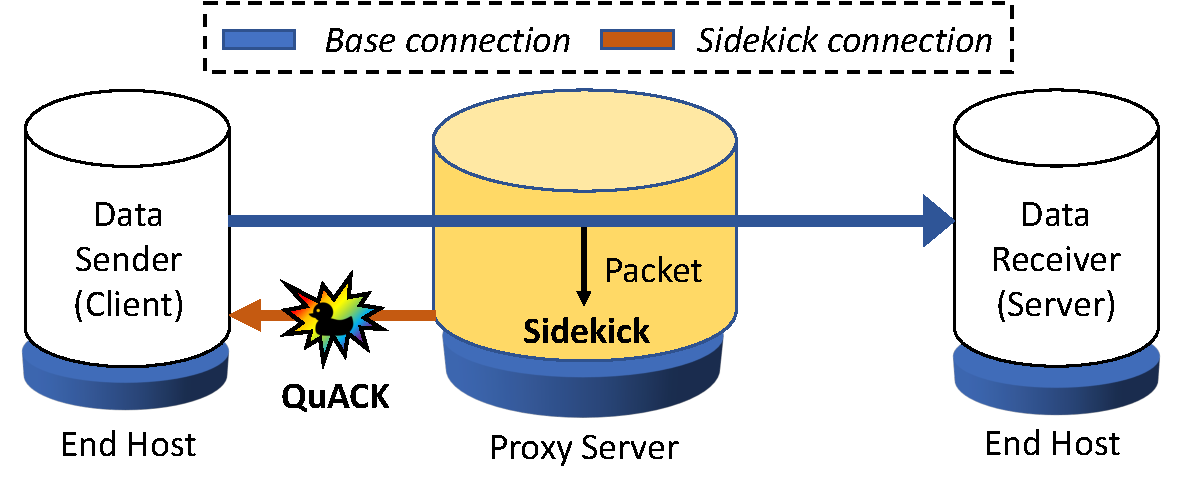
\includegraphics[width=\linewidth]{figures/sc_protocol.pdf}%
\caption{The proxy generates quACKs, in-network acknowledgments, based on
the opaque packets it observes in the base protocol. It quACKs to an end
host, the data sender, which sends or resends packets on the base protocol as a result.
Although we only show one side of the connection, the \sys could assist
either end host of a bidirectional flow.
\vspace{-0.4cm}
}
\label{fig:sc-protocols}
\end{figure}


%What could an end host learn from acknowledgments that originate in
%the \emph{middle} of the connection?
%The end host learns which packets have been lost and received, just like from
%end-to-end ACKs, but it also learns \emph{where} on the path these events have
%occurred.
% We call this acknowledgement from the proxy a \emph{quACK}.
%Unlike a traditional PEP, which reads and interprets the packets
%of an end-to-end connection, sometimes interposing on the connection itself,
%a quACK-sending \sys enables the \emph{end host} to make performance-enhancing
%decisions based on the particulars of the network path.
% make path-aware decisions, \emph{without} violating the end-to-end principle.

%Knowing where on the path packets are lost and received is a powerful tool:
%The end host can
%update the congestion window with knowledge of where the loss occurred,
%retransmit lost packets sooner than detected by end-to-end ACKs,
%and move the sending window in lieu of energy-draining end-to-end ACKs.
%(Forgetting packets in the retransmission buffer is best left to end-to-end
%ACKs given the consequences of being unable to retransmit a lost packet.)
%We motivate the \sys protocol with three scenarios that highlight each of these
%use cases for in-network acknowledgments (\Cref{sec:motivation}).
%\gina{Describe motivating scenarios in more detail in the intro? See: early
%  retransmission over partly-lossy paths, proxy acknowledgments to save energy,
%  and a congestion-control technique to emulate a ``split'' connection by
%  considering where loss occurred along a path.}

%A key technical challenge that has to be solved to enable the \sys protocol
%is the following: \textbf{what is in a quACK and how do we decode it?}
%That is, if sequence numbers are opaque to a PEP, then how can a
%\sys protocol usefully refer to the packets of the underlying transport protocol
%in a way the host can understand?
% More specifically: \textbf{how can a PEP efficiently express a
%   ``cumulative ACK + selective ACK'' over encrypted sequence numbers?}

%We present an efficient construction of the quACK based on the insight that we
%can model the problem as a system of
%power sum polynomial equations when we have a bound on the maximum number of
%missing elements (\Cref{sec:quack}). The power sum quACK enables
%the \sys to transfer the \emph{least} amount of data for the endpoint to
%\emph{efficiently} decode \emph{exactly} which packets have been received.
%We microbenchmark our highly-optimized implementation of the mathematical
%tool to demonstrate its practicality, building on related
%theoretical work of the algebraic technique~\cite{eppstein2011straggler,minsky2003set,karpovsky2003data}.

% One meaningful contribution of our QUIC integration is a modification to the
% CUBIC congestion control algorithm that uses knowledge of \emph{where} loss
% occurs.
%Another interesting technical challenge is how to use knowledge of \emph{where}
%loss occurs to improve congestion control while remaining fair.
%We present a \emph{path-aware} modification
%to the CUBIC congestion control algorithm~\cite{ha2008cubic}
%called \textbf{PACUBIC},
%updating the congestion window proportionally to the
%number of bytes in-flight on the path segment of the congestion event.
%While the congestion behavior of PACUBIC is able to emulate that
%of connection-splitting TCP PEPs, its decisions are made at the end host.

%In the rest of this paper, we describe Robin, our design and implementations
%of the \sys protocol (\Cref{sec:design,sec:implementation}). We implement a
%library for the quACK mathematical tool and a
%\sys binary that sniffs packets and sends quACKs.
%We integrate Robin with two base protocol clients: a simple media client for
%low-latency streaming and an HTTP/3 client
%based on \texttt{libcurl}~\cite{libcurl}
%and a production implementation of QUIC from Cloudflare called \texttt{quiche}~\cite{quiche}.

% We believe that many scenarios would benefit from a \sys protocol,
% allowing the next generation of secure
% transport protocols (including QUIC) to match the performance of
% PEP-accelerated TCP, without compromising their security and privacy
% or promoting ossification. In this paper, we describe several of these
% scenarios and quantitatively evaluate one of them.

% \subsection*{Summary of results}

%We compare these base protocols both with Robin and with end-to-end
%mechanisms alone, and evaluate their performances in our motivating scenarios
%(\Cref{sec:evaluation}).
%In emulation, Robin is able to increase goodput 3.6$\times$, reduce tail latency
%22$\times$, and send 25$\times$ fewer packets at the data receiver in each
%scenario, respectively.
%We show that PACUBIC matches
%the fairness of connection-splitting TCP PEPs, and the \sys
%can process up to 183k packets/s on a single core while sending less than 3\%
%additional packets on the link to the data sender.
%We demonstrate that Robin is robust in a real-world environment with a
%lossy Wi-Fi link and a high-latency cellular path segment.
%Finally, we conclude (\Cref{sec:conclusion}).
% We believe this work does not raise substantial ethical issues.
